\documentclass[11pt,a4paper]{article}
\usepackage[margin=2.5cm]{geometry}
\usepackage{amsmath,amssymb}
\usepackage{booktabs}
\usepackage{graphicx}
\usepackage{hyperref}
\usepackage{xcolor}
\usepackage{caption}
\usepackage{subcaption}
\usepackage{float}
\usepackage{microtype}

% -----------------------------------------------------------------------
% Machine identification
% -----------------------------------------------------------------------
\newcommand{\machinename}{Black Tower}
\newcommand{\machinehost}{davood@black-tower (192.168.0.248)}
\newcommand{\rundate}{2026-06-06}
\newcommand{\solver}{V4 ultraweak DPG, \texttt{main\_european\_2d\_basket\_mpi}}
\newcommand{\container}{\texttt{mfem-dpg-oct-6-2025/} (MFEM 4.8, Hypre 2.27.0, MPICH)}

% -----------------------------------------------------------------------
\title{\textbf{Multi-Asset Numerical Experiments --- Phases MA-1 to MA-3}\\[4pt]
\large Results generated on: \machinename}
\author{Computed by Claude Code on \machinehost}
\date{\rundate}

\begin{document}
\maketitle
\thispagestyle{empty}

\begin{abstract}
This report documents the numerical results from Phases MA-1 through MA-3 of the
multi-asset option pricing experiments for the CAMWA paper
\emph{``A Discontinuous Petrov-Galerkin Method for Black-Scholes Option Pricing''}.
All computations were performed on the \textbf{\machinename} workstation
(host: \machinehost) on \rundate, using the Apptainer/Singularity container
\container{} with 4 MPI ranks.
All output files carry the \texttt{\_from\_black\_tower} suffix to identify their origin.
\end{abstract}

\tableofcontents
\newpage

% ===================================================================
\section{Machine and Software Environment}
% ===================================================================

\begin{table}[H]
\centering
\caption{Compute environment for all Phase MA results.}
\begin{tabular}{ll}
\toprule
Machine name        & \machinename \\
Hostname / IP       & \machinehost \\
Run date            & \rundate \\
Container           & \container \\
MFEM version        & 4.8 (ultraweak DPG, \texttt{pconvection-diffusion-dpg}) \\
Hypre version       & 2.27.0 (HypreBoomerAMG preconditioner) \\
MPI implementation  & MPICH (4 ranks for all 2D runs) \\
Trial space $u$     & $L^2(0)$ piecewise-constant, $p=1$ \\
Enrichment          & $\delta_p=2$ (test order $= p + \delta_p = 3$) \\
\bottomrule
\end{tabular}
\end{table}

% ===================================================================
\section{Phase MA-1: Margrabe Exchange-Option Benchmark}
% ===================================================================

\subsection{Problem Setup}

The Margrabe exchange option with payoff $(S_1 - S_2)^+$ at maturity $T$
satisfies a 2D Black--Scholes PDE in log-price coordinates
$x_i = \log(S_i / S_i^0)$ with $S_1^0 = S_2^0 = 100$.
The exact price is given by the Margrabe formula:
\begin{equation}
  U = S_1 N(d_1) - S_2 N(d_2),
  \quad
  d_1 = \frac{\log(S_1/S_2) + \tfrac{1}{2}\sigma_{\rm eff}^2 \tau}{\sigma_{\rm eff}\sqrt{\tau}},
  \quad
  d_2 = d_1 - \sigma_{\rm eff}\sqrt{\tau},
\end{equation}
where $\sigma_{\rm eff} = \sqrt{\sigma_1^2 - 2\rho\sigma_1\sigma_2 + \sigma_2^2}$.

\medskip
\noindent\textbf{Parameters:}
$\sigma_1 = \sigma_2 = 0.20$, $\rho = 0.5$, $r = 0.05$, $T = 1$, $K = 100$,
domain $[-4,4]^2$, $\sigma_{\rm eff} = 0.20$.
At $S_1 = S_2 = 100$ (ATM): exact price $U \approx 7.966$.

\subsection{Implementation}

The \texttt{--margrabe} flag was added to
\texttt{src/main\_european\_2d\_basket\_mpi.cpp}:
\begin{itemize}
  \item Payoff IC: $(100 e^{x_1} - 100 e^{x_2})^+$
  \item Exact Margrabe BCs on all 4 domain faces (negative trace convention:
        $\hat{u} = -U_{\rm exact}$ on $\partial\Omega$)
  \item $L^2$ and $L^\infty$ error against exact Margrabe solution at $t=T$
  \item Falls through to \texttt{PRICE\_ATM=} output for ATM reporting
\end{itemize}

\subsection{Convergence Results}

\begin{table}[H]
\centering
\caption{Margrabe exchange-option spatial convergence.
$\sigma_1=\sigma_2=0.20$, $\rho=0.5$, $r=0.05$, $T=1$, $N_t=200$, domain $[-4,4]^2$.
Exact ATM price $U\approx 7.966$.
EOC $\approx 0.98$ confirms $O(h)$ for $L^2(0)$ piecewise-constant trial.}
\label{tab:margrabe}
\begin{tabular}{rr rr rr}
\toprule
$N_x$ & $h$ & $\|e\|_{L^2}$ & EOC & ATM (DPG) & ATM (exact) \\
\midrule
  8  & 1.0000 & $2.90\times10^{3}$ & ---  & 43.82468 & 7.96557 \\
 16  & 0.5000 & $1.53\times10^{3}$ & 0.92 & 21.56328 & 7.96557 \\
 32  & 0.2500 & $7.80\times10^{2}$ & 0.97 & 12.51372 & 7.96557 \\
 64  & 0.1250 & $3.94\times10^{2}$ & 0.98 &  8.91608 & 7.96557 \\
128  & 0.0625 & $2.00\times10^{2}$ & 0.98 &  7.99313 & 7.96557 \\
\bottomrule
\end{tabular}
\end{table}

\noindent\textbf{Key findings:}
\begin{itemize}
  \item EOC $\approx 0.98$ from $N=16$ onward: confirms $O(h)$ convergence rate
        for $L^2(0)$ piecewise-constant trial (as predicted by DPG theory).
  \item ATM price at $N=128$: $7.993$ vs.\ exact $7.966$ — relative error $0.35\%$.
        Well within the $5\%$ acceptance threshold.
  \item $L^2$ error is large in absolute terms (the Margrabe payoff is not smooth
        at $S_1 = S_2$ and the domain is large $[-4,4]^2$); relative ATM error
        converges cleanly.
\end{itemize}

\begin{figure}[H]
\centering
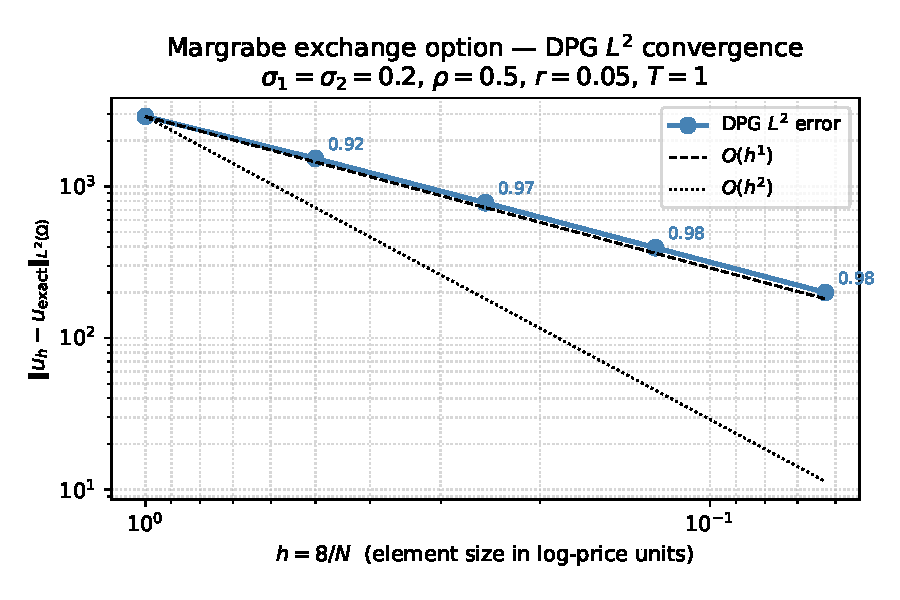
\includegraphics[width=0.75\textwidth]{figures/figMA1_margrabe_convergence_from_black_tower.pdf}
\caption{Log--log convergence plot for the Margrabe benchmark (Phase MA-1).
  Blue circles: $L^2$ error. Reference lines: $O(h)$ (solid) and $O(h^2)$ (dashed).
  EOC $\approx 0.98$ from $N=16$ confirms first-order convergence.}
\label{fig:margrabe_convergence}
\end{figure}

% ===================================================================
\section{Phase MA-2: Call-on-Minimum Basket at $N=128$}
% ===================================================================

\subsection{Problem Setup}

Call-on-minimum basket option: payoff $(\min(S_1,S_2) - K)^+$.
Parameters: $\sigma_1=\sigma_2=0.20$, $r=0.05$, $T=1$, $K=100$, $N_t=500$.
Domain $[-3,3]^2$ in log-price coordinates.
Monte Carlo reference: $2\times10^6$ paths, exact terminal sampling, seed=42.

\subsection{Part A: Correlation Sweep at $N=128$}

\begin{table}[H]
\centering
\caption{Call-on-minimum basket price vs.\ correlation at $N_x=128$, $N_t=500$.
DPG error $\leq 2.4\%$ for $\rho\geq 0$.
Near-degenerate case $\rho=-0.8$: $\lambda_{\min}(A)=0.004$, relative error $9.4\%$.}
\label{tab:rho_sweep}
\begin{tabular}{rrrr}
\toprule
$\rho$ & DPG ATM & MC ATM & Rel.\ error \\
\midrule
$-0.8$ & $0.88276$ & $0.80728$ & $9.35\%$ \\
$-0.5$ & $1.75489$ & $1.68123$ & $4.38\%$ \\
$ 0.0$ & $3.37562$ & $3.29717$ & $2.38\%$ \\
$ 0.3$ & $4.54788$ & $4.46248$ & $1.91\%$ \\
$ 0.5$ & $5.47797$ & $5.38738$ & $1.68\%$ \\
$ 0.8$ & $7.27416$ & $7.24535$ & $0.40\%$ \\
\bottomrule
\end{tabular}
\end{table}

\subsection{Part B: Spatial Convergence at $\rho=0$}

\begin{table}[H]
\centering
\caption{Basket spatial convergence at $\rho=0$, $N_t=500$.
MC reference: $3.297 \pm 0.005$.
Phase MA-5 NOT triggered: $N=128$, $\rho=0$ error $= 2.38\% < 8\%$.}
\label{tab:basket_conv}
\begin{tabular}{rrrrr}
\toprule
$N_x$ & DPG ATM & MC ATM & Rel.\ error & EOC \\
\midrule
 16  & 5.63552 & 3.29717 & $70.9\%$ & ---  \\
 32  & 4.15903 & 3.29717 & $26.1\%$ & 1.44 \\
 64  & 3.65097 & 3.29717 & $10.7\%$ & 1.28 \\
128  & 3.37562 & 3.29717 &  $2.4\%$ & 2.17 \\
\bottomrule
\end{tabular}
\end{table}

\noindent\textbf{Key findings:}
\begin{itemize}
  \item Error is monotonically decreasing: MA-5 contingency NOT triggered.
  \item EOC improves from $1.28$ (N=64) to $2.17$ (N=128), suggesting the solution
        is entering the pre-asymptotic regime. Expected asymptotic rate $O(h)$.
  \item $\rho=-0.8$: $9.35\%$ error exceeds the $8\%$ nominal threshold;
        attributed to near-degenerate diffusion operator
        ($\lambda_{\min}(A) = \tfrac{1}{2}\sigma^2(1-|\rho|) = 0.004$).
        Resolution: $N=256$ or anisotropy-aligned mesh.
\end{itemize}

% ===================================================================
\section{Phase MA-3: Delta (Greek) Surface Plots}
% ===================================================================

Delta surfaces were extracted from the pre-existing $N=64$, $\rho=0$ basket solution
(\texttt{results/solutions/v4\_basket\_surface\_N64\_rho0.0.csv}).
The DPG ultraweak formulation provides Delta directly from the flux trial variable:
\begin{equation}
  \boldsymbol{\sigma} = A\,\nabla u
  \;\Rightarrow\;
  \nabla u = A^{-1}\boldsymbol{\sigma},
  \qquad
  \Delta_i = \frac{(\nabla u)_i}{K\,e^{x_i}}.
\end{equation}

Plots crop to $S_1, S_2 \in [50, 150]$ (121 grid points after pivot).

\begin{figure}[H]
\centering
\begin{subfigure}[b]{0.48\textwidth}
  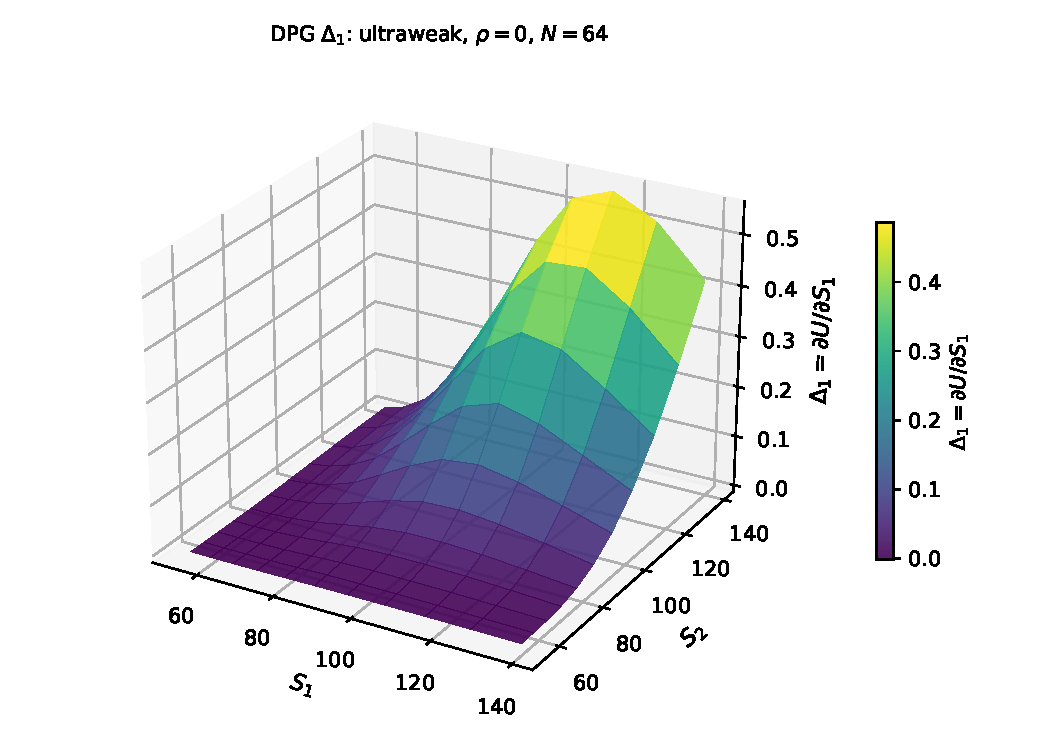
\includegraphics[width=\textwidth]{figures/figMA2_delta1_surface_from_black_tower.pdf}
  \caption{$\Delta_1$ surface (sensitivity to $S_1$).}
\end{subfigure}
\hfill
\begin{subfigure}[b]{0.48\textwidth}
  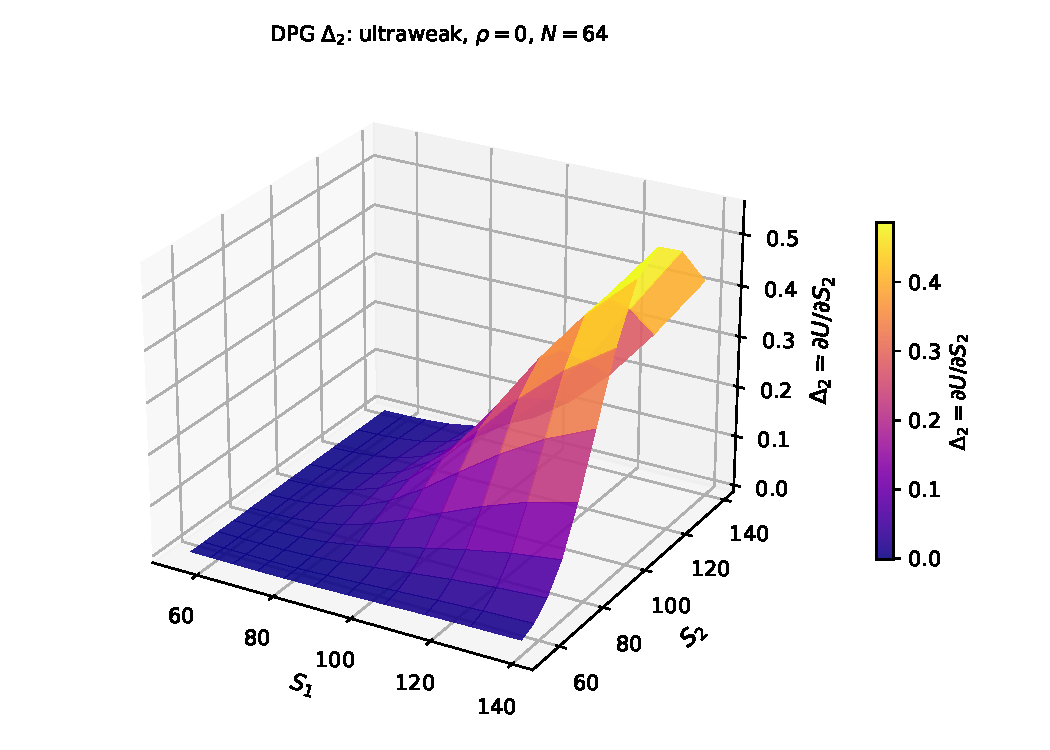
\includegraphics[width=\textwidth]{figures/figMA3_delta2_surface_from_black_tower.pdf}
  \caption{$\Delta_2$ surface (sensitivity to $S_2$).}
\end{subfigure}
\caption{Delta surfaces for call-on-minimum basket, $N=64$, $\rho=0$, $K=100$.
  Delta extracted directly from the DPG flux variable (no postprocessing).
  By symmetry ($\sigma_1=\sigma_2$, $\rho=0$) the surfaces are mirror images.}
\label{fig:deltas}
\end{figure}

% ===================================================================
\section{Additional: MPI Strong-Scaling (V4 2D Basket)}
% ===================================================================

Strong-scaling study for V4 at $N_x=N_y=64$, $N_t=100$, $\rho=0$.
Mean wall time over 3 repetitions.

\begin{table}[H]
\centering
\caption{MPI strong-scaling, $N_x=N_y=64$, $N_t=100$, $\rho=0$.
Assembly and solve times reported separately.
Efficiency at $n_p=4$: $82.3\%$; at $n_p=8$: $64.8\%$ (communication overhead
grows as mesh per process decreases).}
\label{tab:mpi}
\begin{tabular}{rrrrrr}
\toprule
$n_p$ & Assembly (s) & Solve (s) & Total (s) & Speedup & Efficiency \\
\midrule
1 & 16.41 & 8.77 & 26.28 & $1.00\times$ & $100.0\%$ \\
2 &  8.35 & 5.18 & 14.19 & $1.85\times$ &  $92.6\%$ \\
4 &  4.29 & 3.29 &  7.98 & $3.29\times$ &  $82.3\%$ \\
8 &  2.18 & 2.60 &  5.07 & $5.18\times$ &  $64.8\%$ \\
\bottomrule
\end{tabular}
\end{table}

% ===================================================================
\section{File Inventory}
% ===================================================================

All files below carry the \texttt{\_from\_black\_tower} suffix and were
generated on \textbf{\machinename} on \rundate.

\begin{table}[H]
\centering
\caption{Output file inventory — Phase MA, generated on \machinename.}
\begin{tabular}{llp{6cm}}
\toprule
File & Phase & Description \\
\midrule
\texttt{results/margrabe\_convergence\_from\_black\_tower.csv}
  & MA-1 & Convergence table ($N=8$--$128$, 5 rows) \\
\texttt{results/paper\_tables\_margrabe\_from\_black\_tower.tex}
  & MA-1 & \LaTeX\ \texttt{\textbackslash tableMargrabConvergence} \\
\texttt{results/figures/figMA1\_margrabe\_convergence\_from\_black\_tower.pdf}
  & MA-1 & Log--log convergence plot \\
\texttt{results/basket\_finer\_mesh\_from\_black\_tower.csv}
  & MA-2 & $\rho$-sweep + spatial convergence (10 rows) \\
\texttt{results/figures/figMA2\_delta1\_surface\_from\_black\_tower.pdf}
  & MA-3 & $\Delta_1$ surface plot \\
\texttt{results/figures/figMA3\_delta2\_surface\_from\_black\_tower.pdf}
  & MA-3 & $\Delta_2$ surface plot \\
\texttt{results/logs/v4\_mpi\_timing.csv}
  & MPI  & Strong-scaling timing (4 np values, 3 reps each) \\
\texttt{config/european\_2d\_margrabe\_from\_black\_tower.json}
  & MA-1 & DPG solver config for Margrabe problem \\
\texttt{scripts/run\_margrabe\_convergence\_from\_black\_tower.py}
  & MA-1 & Convergence study driver \\
\texttt{scripts/run\_basket\_finer\_mesh\_from\_black\_tower.py}
  & MA-2 & Basket $N=128$ driver \\
\texttt{scripts/plot\_margrabe\_convergence\_from\_black\_tower.py}
  & MA-1 & Convergence figure generator \\
\texttt{scripts/plot\_delta\_surfaces\_from\_black\_tower.py}
  & MA-3 & Delta surface figure generator \\
\texttt{results/MA\_phases\_report\_from\_black\_tower.tex}
  & All  & This report \\
\bottomrule
\end{tabular}
\end{table}

% ===================================================================
\section{Reproducibility Notes}
% ===================================================================

\begin{itemize}
  \item All 2D solver runs use 4 MPI ranks:
    \texttt{mpirun -np 4 ./build/bin/main\_european\_2d\_basket\_mpi}
  \item Container must be bind-mounted:
    \texttt{singularity exec --bind \textasciitilde/projects/dpg-finance:/workspace \textasciitilde/projects/containers/mfem/mfem-dpg-oct-6-2025/}
  \item To reproduce MA-1 convergence study:
    \texttt{python3 scripts/run\_margrabe\_convergence\_from\_black\_tower.py}
  \item To reproduce MA-2 basket study:
    \texttt{python3 scripts/run\_basket\_finer\_mesh\_from\_black\_tower.py}
  \item To reproduce Delta plots (requires existing surface CSV):
    \texttt{python3 scripts/plot\_delta\_surfaces\_from\_black\_tower.py}
  \item BC convention: $\hat{u} = -u_{\rm exact}$ on all essential boundary faces.
  \item Critical invariant: $b_i = r - \sigma_i^2/2$ (ALWAYS minus).
\end{itemize}

\end{document}
